\begin{figure}[t]\centering
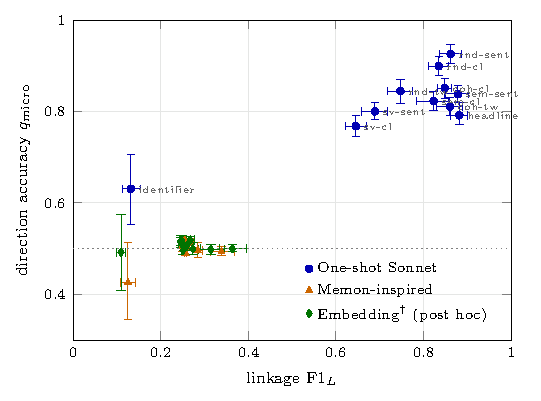
\includegraphics[width=\linewidth]{FIGURES/fig3.pdf}
\caption{Linkage vs ordering decomposition: linkage component F1\textsubscript{L} (mean, 95\% CI) against micro-averaged direction accuracy q (95\% CI), by condition. F1\textsubscript{J} = F1\textsubscript{L} $\times$ q. Dotted line: q = 0.5 (chance direction). Labels: rnd = random, sem = semantic, coh = coherence-sever, sv = subject-verb; sent = sentence, cl = clause, tw = token-window.}
\label{fig:3}
\end{figure}
